% This is samplepaper.tex, a sample chapter demonstrating the
% LLNCS macro package for Springer Computer Science proceedings;
% Version 2.20 of 2017/10/04
%
\documentclass[runningheads]{llncs}
%
\usepackage{graphicx}
% Used for displaying a sample figure. If possible, figure files should
% be included in EPS format.
%
% If you use the hyperref package, please uncomment the following line
% to display URLs in blue roman font according to Springer's eBook style:
% \renewcommand\UrlFont{\color{blue}\rmfamily}

\begin{document}
%
\title{Semi-supervised sentiment analysis for Chinese stock texts in scarce labeled data scenario and price prediction\thanks{Peking University Grant 2020: "New Ideas for Teaching 2.0" Key Project; MSTC
Grant 2019: research, development and demonstration of key technologies for knowledge organization and services for antiques based on Knowledge Graph; NSFC Grant 61772044}}
%
%\titlerunning{Abbreviated paper title}
% If the paper title is too long for the running head, you can set
% an abbreviated paper title here
%
\author{Ji Zhaoyan\inst{1} \and
Yan Hongfei\inst{1,3}\orcidID{0000--0001--5914--8585} \and
Ying Siping\inst{1}\orcidID{[0000--0001--5829--1865} \and
Chen Chong\inst{2}\orcidID{0000--0002--9704--1575} \and 
Su Qi\inst{1}\orcidID{0000--0002--4769--2812}}
%
\authorrunning{F. Author et al.}
% First names are abbreviated in the running head.
% If there are more than two authors, 'et al.' is used.
%
\institute{Peking University, Beijing, P.R.China \email{\{zhaoyanji,yanhf,sukia\}@pku.edu.cn} 
\email{spying@gmail.com}\and
Beijing Normal University \email{chenchong@pku.edu.cn} \and
National Engineering Laboratory for Big Data Analysis and Application
Technology, Center for Big Data Research, Peking University, Beijing, P.R.China}
%
\maketitle              % typeset the header of the contribution
%
\begin{abstract}
The application of neural network in stock prediction is developing rapidly these years because of its excellency in series data processing. However, as most of research are conducted in English, data sources and labeled data are inadequate in Chinese. Especially for natural language processing tasks in specific domain where specialized labeled data are required to train models to adapt to terminology processing, specialized labeled Chinese in text data are very scarce, such as financial text data. To tackle this challenge, we proposed a semi-supervised learning method to generate well-labeled data and train BERT, a leading natural language processing model, to obtain a trained sentiment machine. Then we got stock-related text data sentiment score based on this machine and further combine the sentiment score and other transaction data as inputs for different neural networks to predict stock price. The experimental results on a large scale of Chinese stock data and texts showed that our proposed method successfully improved prediction accuracy compared to other established methods. Besides, we also examined our method's applicability combined with different neural networks when predicting different types of stock.
\keywords{stock prediction  \and sentiment analysis in scarce labeled data domain \and deep neural networks}
\end{abstract}
%
%
%
\section{Introduction}
Stock market is an efficient way for companies to raise funds and for investors to generate financial returns. These advantages led stock market become a critical part of national economies. As stock becomes more and more inseparable to our life, precisely predicting stock price gradually draws scholars' attention. However, stock price changes in a volatile and chaotic way, resulting in dysfunction of lots of prediction methods. As deep neural network evolves and displays a extraordinary performance in times series data processing, it was frequently put into use in stock prediction tasks and generated relatively accurate results.

However, previous research was concentrated in English domain and lack of presence in Chinese, which caused the insufficiency of Chinese data source and labeled data accumulation. This problem becomes severely influential in natural language processing tasks in specific domain because specialized labeled data are needed for model training to identify and process terminology. Therefore, natural language processing related tasks in specific domain such as sentiment analysis faces a great challenge in Chinese.
In this passage, we propose a semi-supervised learning method to tackle the problem of lack of Chinese labeled data in financial texts. We first crawled stock-related text data from a Chinese leading professional transaction website. We evaluated the sentiment score of those text data based on a naive sentiment model trained by general data. Then, we identified the ambiguous text with complex information and adjusted it manually. Based on this method, we successfully generated a batch of well-labeled data and further applied it into the fine-tuning of a leading NLP model, BERT, and managed to improve its performance in financial domain significantly.

In order to test this method's efficiency, we combined this sentiment analysis method into a stock prediction model in which we used sentiment score and transaction data to predict future close price for a certain stock.The specific problem can be defined as below:

Given a certain stock s and arbitrary trading day t, its close price can be predicted by a time series of its historical information of length T $[t-T,...,t-1]$. The information will include transaction data $[V_{t-T}^s,...,V_{t-1}^s]$ and text data $[W_{t-T}^s,...,W_{t-1}^s]$. The equation goes like below:
\begin{equation}
\hat{p}_t^s = f([V_{t-T}^s, ..., V_{t-1}^s], [W_{t-T}^s,...,W_{t-1}^s])
\end{equation} 

Following this definition, we combined the sentiment score with transaction data obtained from financial database and put them into prediction models. We used several neural networks as our prediction model to test our method's efficiency and performance characteristic on different neural network structure. 

The experimental results further proved our method's efficiency and applicability in stock prediction field. Besides, it can generate different performance combined with different neural networks when predicting different type of stocks.

The rest of the paper will be organized as follows. Section 2 will introduce several related works. Section 3 will proceed with framework and details of our model. Section 4 will display the experimental results that directly show our method's efficiency. Section 5 will end with a conclusion of our work in this passage.

\section{Related Works}
Computer technology have long been adopted in stock prediction throughout its development history. After the birth of neural networks, the development of computer empowered stock prediction begin to accelerate. The neural networks show great excellency in series data processing which can be used both in stock transaction data processing and stock related text data analyzing. Based on financial domain knowledge, the stock prediction method can be categorized into three main segments.

The first segment is technical analysis driven prediction. This method believed market will repeat its behavior in a certain pattern. Therefore, they based their method on analyzing market data to discover the underlying patterns. The MACD~\cite{MACD} method, brought up by Gerald Appel, is a classical representation. They used stock's average price over different time span as an indicator to capture its future trend. Computer technology is, therefore, more adequate for this problem because of its superiority in handling data and capturing subtle trends. It made the first breakthrough after the 
application of auto-regression~\cite{autoregression} model. Several scholars revised this model using machine learning techniques like SVM~\cite{ML-autoregression} to capture stock price's volatility. However, those methods still weren't able to capture the high volatility and chaotic. The neural network showed outstanding performance dealing those problem and therefore was put into use soon after its releasing. Among neural network frameworks, recurrent neural network displayed the highest capability~\cite{neuralnetwork} because its structure was specifically designed for time series data prediction. Later researchers have made several revisions on top of the RNN structure to make it more specific for stock prediction. Hu~\cite{SFM} et al. proposed a State-Frequency Memory network in a recent work. They added a Fourier Transformation in LSTM cells to distinguish long term and short term indicators for stock price trend. 

The second segment is fundamental analysis driven prediction. This method based its prediction on the analysis of the intrinsic value of a company implied by its operating performance. The dependence of company inside information and unstructured analysis constraint computer technology performance as compared to human investors with abundant domain knowledge. But still, there are some researchers managed to find proxies for computer to discover insights using a computation method. Chen et al.~\cite{investmentbev} used mutual fund's portfolio data as a proxy for investment manger's stock preference. Their research proceeded with the assumption that stock held the same investor share same intrinsic properties, and therefore they were able to undermine inside information by leveraging public mutual fund portfolio data.

The third segment is information driven prediction. Text data such as news, announcements, and stock comments are used in this method to reveal stock's property and investors' sentiment. Neural networks are crucial to this method because it not only make precise prediction for time series data but also powerful in handling text data. Ding et al.~\cite{dlnews} proposed a deep learning driven method to extract stock-related information from news and further predict stock price. Furthermore, neural network driven sentiment analysis can also be adopted into stock prediction by evaluating investors' sentiment through their comments because advanced financial research found out that investor sentiment can also affect stock price. Si et al.~\cite{sentimentprediction} have used comments extracted from tweets to derive sentiment score and used it to predict stock price. In later research, scholars used financial specific labeled data to train BERT~\cite{finbert}, a state-of-the-art NLP technique, and obtained an outstanding performance in financial text sentiment analysis, successfully improving prediction accuracy. 

However, as most of the research are conducted in English background, Chinese stock prediction research are relatively rare, especially the method based on sentiment analysis. The insufficiency of research results in the lack of accumulation of Chinese data source and labeled data, which obstruct future generation of scholars to deep dive into this area. Our passage proposed a method to generate labeled data in a semi-supervised way and solve the problem once and for all. 

\section{Method}

Inspired by Dasgupta's method~\cite{semi-supervised} of semi-supervised learning in scarce labeled data environment by categorizing data into groups and manually adjusting ambiguous group, we adopted a similar semi-supervised process to handle unlabeled text data for stocks. Then we generated labeled data and put them into BERT to obtain a well-established sentiment machine. We further derived sentiment score using this machine and combine the score with transaction data. Finally we run several neural network models with combined data as input to train prediction model. The overall framework is displayed bellow.
\begin{figure}
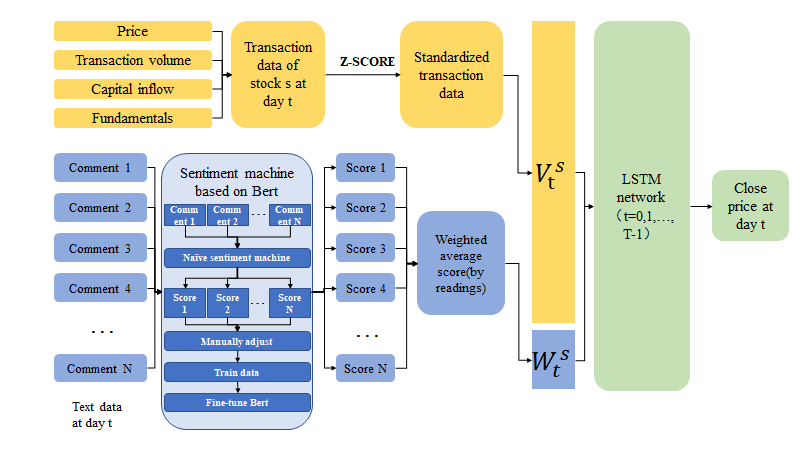
\includegraphics[width=\textwidth]{model-en.png}
\caption{Framework} \label{fig1}
\end{figure}

\subsection{Framework}
As showed in the above framework, the proposed is model mainly composed of three layers:
\begin{itemize}
    \item Text data processing layer: crawled data from a specific source to get abundant Chinese data sources. Trained the sentiment machine based on semi-supervised method to evaluate each texts and deliver their sentiment score.
    \item Transaction data processing layer: get four types of transaction data and standardized it to improve prediction performance.
    \item Prediction layer: adopted several neural network models to testify our method's efficiency and adaptability. 
\end{itemize}

\subsection{Text data processing}

We used a leading Chinese online stock transaction platform Eastmoney as our text data sources. This website preserved lots of text information of company news and investor comments across a long time span as examples showed in fig.\ref{fig:eastmoney}. We applied a web-crawler technology here and a proxy IP tactic to successfully get 1.05M text data from 6 different stocks in each trading day between 2010 and 2020.
\begin{figure}
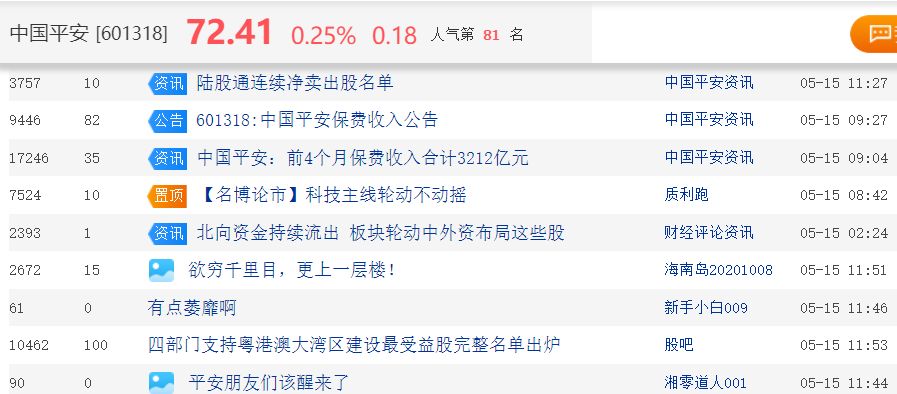
\includegraphics[width=\textwidth]{pingacomment.png}
\caption{Text data source} \label{fig:eastmoney}
\end{figure}
Then, we extract a batch of the raw text data as unlabeled train data. Firstly, we applied a naive sentiment machine trained on general Chinese data source mainly composed of comments from e-commerce website. Then we identified ambiguous text by matching raw data with stock terminology database. By this way, we filtered out a group of ambiguous text because of terminology. After manually adjusted, the ambiguous text's sentiment score became clear and qualified for being training data for the final sentiment machine. We combine the adjusted ambiguous group and the unambiguous group together to train BERT-Chinese model to obtain a accurate sentiment machine for stock comments and news. We tested the accuracy of the trained machine on testing data set and compared the result with the naive sentiment machine. The result in table.\ref{tab:sentimentcomps} shows our method significantly improved the sentiment analysis accuracy.
\begin{table}
    \centering\caption{Sentiment analysis accuracy comparison}\label{tab:sentimentcomps}
    \begin{tabular}{|l|l|}
        \hline
        Method &  Accuracy\\
        \hline
        Trained BERT & 88.2\%\\
        Naive Sentiment Machine & 80.27\%\\
        \hline
    \end{tabular}
\end{table}

Considered that different text have different level of influence on market sentiment, we adopted a weighted average method to calculate the sentiment score of a certain trading day $t$. Because the influence level of each text can be represented by its readings, which is recorded by the Eastmoeny website we chose. Therefore, we used the reading as weight to average the sentiment score of a certain trading day as showed in the following equation. We used all data(i=1,2,...,N) of a certain day t to calculate the weighted average $sentiment_t^s$. Finally, we passed each trading day's sentiment score and reading to the prediction layer.
\begin{equation}
    sentiment_t^s = \frac{\Sigma_{i=1}^{N}sentiment_t^{si}*reading_t^{si}}{\Sigma_{i=1}^Nreading_t^{si}}
\end{equation}

\subsection{Transaction data processing}
We first get stock transaction data from a established Chinese financial database. We chose different types of stock in terms of industry and historical performance and collected data from 2010 to 2020 on each trading day. Specifically, we collected following four types of data:
\begin{itemize}
    \item Price information: include the starting price, the close price, daily highest price and daily lowest price. reveals stock price's volatility.
    \item Volume information: include transaction volume, turnover rate and circulation market value. reveals investors transaction enthusiasm.
    \item Capital flow information: include net capital flow from mega size, large size, medium size and small size transaction. reveals different type of investors' different preference of holding a stock.
    \item Fundamental information: P/B and P/S ratio. reveals the stock corresponding company operating performance.
\end{itemize}

The distribution of those data is not united, highly likely to bring chaotic into prediction model. In order to eliminate the negative effect, we adopted Z-Score method to normalize all the input data. Z-Score is showed in the following equation. Then we passed all the normalized data together with data derived from text layer into prediction model.
\begin{equation}
    normInput_t^s = \frac{Input_t^s-\overline{Input^s}}{\sigma_{Input^s}}
\end{equation}

\subsection{Prediction layer}
In this layer, we accepted data inputs from former layers and used them to predict future close price. We applied three different types of neural network to process the data to comprehensively test our method's efficiency.
\begin{itemize}
    \item Multi-Layer Perceptron(MLP): this is the most classical neural network model. It is composed of input layer, hidden layer and output layer. Each layer is fully connected with multiple neural cells activated by non-linear function such as ReLU and sigmoid. Its forward propagation goes like following:
    \begin{equation}
        y_i = \sigma(\sum_{i}W_ix_i+b_i)
    \end{equation}
    \item Long Short Term Memory network(LSTM): this is a upgrade version of recurrent neural network. Introducing input, forget and output gates within each cell, LSTM successfully memorized crucial information from past time steps and used it to supplement current information. LSTM shows an outstanding performance in lots of series data processing fields and is therefore the most frequent used recurrent neural network.
    \item Gated Recurrent Unit(GRU): this is also a upgrade version of recurrent neural network. Similar to LSTM, GRU leverage reset and update gate to memorize past information. However, GRU's structure is simpler than LSTM, and thus easy to converge. Despite of convergence discrepancy, our experiments also discovered that they have different performance facing different type of stocks. 
\end{itemize}


\section{Experiments}
We used Pytorch in Python to train and test our model. Our dataset and experiment results are showed below.
\subsection{Dataset}
To testify our method’s efficiency on handling Chinese data, we obtained our experimental data from Chinese A share. We chose 6 different stocks with different market value, operating performance and industries to prove our method’s adaptability across different stocks. We got their transaction data from 2010/01/01 to 2020/01/01 on each trading day through an established Chinese financial database Tushare. Then, we crawled the corresponding text data from Eastmoney website. The detailed information of those 6 stocks are shown below.
\begin{table}[htbp]
	\renewcommand\arraystretch{1}
	\caption{Stock information}\label{tab:data}
	\begin{tabular}{c|c|c|c|c}
		\hline
		Stock&Stock code&\# days &\# texts&Stock properties\\\hline\hline
		Pingan&601318.SH&2431&337.9K&Finance, big size, high growth\\\hline
		Yili&600887.SH&2447&191.9K&Consumer, big size, stable\\\hline
		Wentai&600745.SH&1989&118.6K&Semi-conductor, medium size, volatile\\\hline
		Changjiang&600887.SH&2369&148.2K&Energy, medium size, cyclical\\\hline
		Yangquan&600348.SH&2477&117.7K&Chemical and Energy, small size, volatile\\\hline
		(ST)Gongxin&600701.SH&2160&142K&Manufacture, small size, poor performance\\\hline
	\end{tabular}
\end{table}

\subsection{Experiment setup}
We adopted different neural network models stated above with different type of data as input. Specifically, we set up our experiment in 4 different ways:
\begin{itemize}
    \item MLP + price data: we used past 30 days close price as input to pass into MLP model with 4 hidden layers and ReLU as activation function which is consistent with other RNN models.
    \item LSTM + transaction data: we used 14-dimension transaction data including price, transaction volume, capital flow and fundamental data. Then we used a LSTM network with a 30 days timestep to accord with MLP for comparison. 
    \item GRU + transaction data: same input as the above LSTM model. We replaced the LSTM layer with GRU to compare their performance.
    \item LSTM + transaction data + text data: we used 16-dimension data combining transaction data and sentiment score and reading together to testify our method’s efficiency.
    \item GRU + transaction data + text data: we replaced the above LSTM layer with GRU layer to expand our method’s adaptability.
\end{itemize}

\subsection{Evaluation Metric}
In order to testify our method's efficiency, we introduced two way to examine the result and cross check with each other to comprehensively understand our experimental results.
The first metric we used is Root Mean Square Error(RMSE) to evaluate the absolute distance between predicted result and real data. It is calculated as bellow:
\begin{equation}
    RMSE(X,h) = \sqrt{\frac{1}{m}\sum_{i=1}^m(h(x_i)-y_i)^2}
\end{equation}

The second way is to directly depict the figure of predicted and real data. By this way, we can visually understand the result revealed by RMSE.

\subsection{Experiment result}
As introduced in the above section, we applied RMSE function as an evaluation metric. The detailed results are shown as below:
\begin{table}
    \renewcommand\arraystretch{1.2}
	\centering\caption{Experiment result}\label{tab:RMSE}
    \begin{tabular}{|c|c|c|c|c|c|c|}
        \hline
        Model&Pingan&Yili&Wentai&Changjiang&Yangquan&(ST)Gongxin\\\hline\hline
        MLP&0.146&0.259&0.748&0.116&0.061&0.039\\\hline
        LSTM\_data& 0.148 & 0.145 & 0.819 & 0.098 & 0.018 & 0.116 \\\hline
        GRU\_data&0.206&0.099&0.825& 0.064& 0.021& 0.050\\\hline
        LSTM\_text+data& 0.148& 0.145& 0.802& 0.096& 0.018& 0.108\\\hline
        GRU\_text+data & 0.057& 0.071& 0.471& 0.102& 0.018& 0.080\\\hline
    \end{tabular}
\end{table}

Based on this experiment result and together with some figure depicted from prediction result, we can derive following arguments:
\begin{itemize}
    \item Our method showed significant efficiency over our experiments: table\ref{tab:RMSE} showed that RMSE decreased after we added sentiment data derived from our proposed method. The improvement was more obvious when combined with GRU model and applied to more volatile stock with higher growth potential. In order to gain a more comprehensive observation on our method, we put stock Pingan and Yili’s result prediction figure below(fig\ref{fig:Pingan}, fig\ref{fig:Yili}). As we can tell from the figure, the RMSE reduction came from more precisely fitting degree between prediction result and real data, especially on sections with high fluctuation. Our method is better at predicting future trend where the comparing method sometimes lagged behind.
    \item LSTM and GRU have different performance on different type of tasks: Through RMSE data, we can tell that those two networks don’t have distinctive advantage over each other on whole scale. LSTM method performed better on high growth and fluctuate stocks such as Wentai and Pingan while GRU performed better on stable stocks such as Yili and Changjiang Electricity. 
    \item MLP is invalid on stock prediction: Although MLP delivered lower RMSE result as shown in the table, fig\ref{fig:MLPres} shows that it just averaged price over a certain time span. This methodology is ineffective in stock prediction field where even subtle trend can be crucial to capture.
\end{itemize}
\begin{figure} 
  \centering 
  \subfigure[Transaction data]{ 
    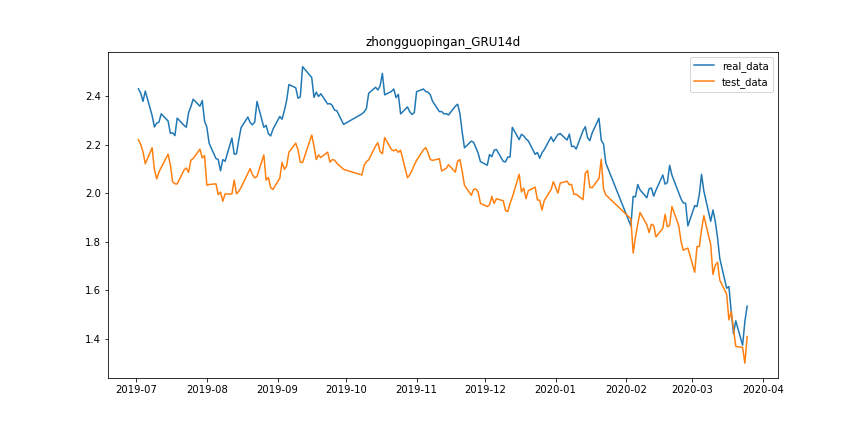
\includegraphics[width=4in]{zhongguopingan_GRU14d.png} 
    \label{fig:pingan_14d} %% label for first subfigure
  } 
  \subfigure[Extend text data]{ 
    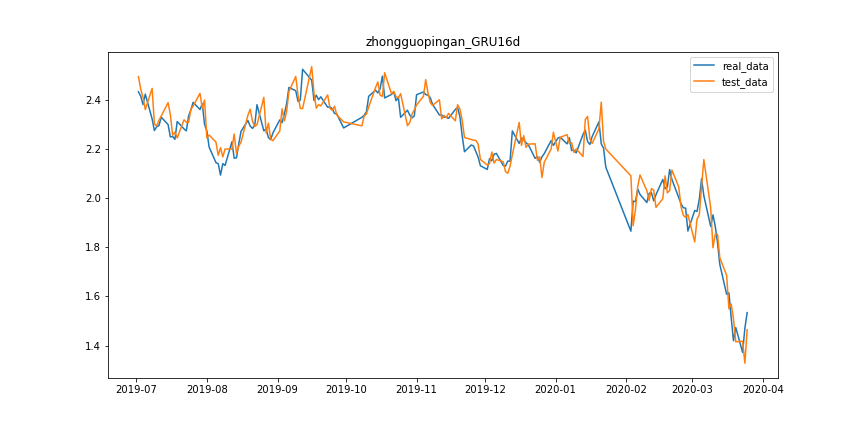
\includegraphics[width=4in]{zhongguopingan_GRU16d.png} 
    \label{fig:pingan_16d} %% label for second subfigure 
  } 
  \caption{Pingan's prediction result} 
  \label{fig:Pingan} %% label for entire figure 
\end{figure}
\begin{figure} 
  \centering 
  \subfigure[Transaction data]{ 
    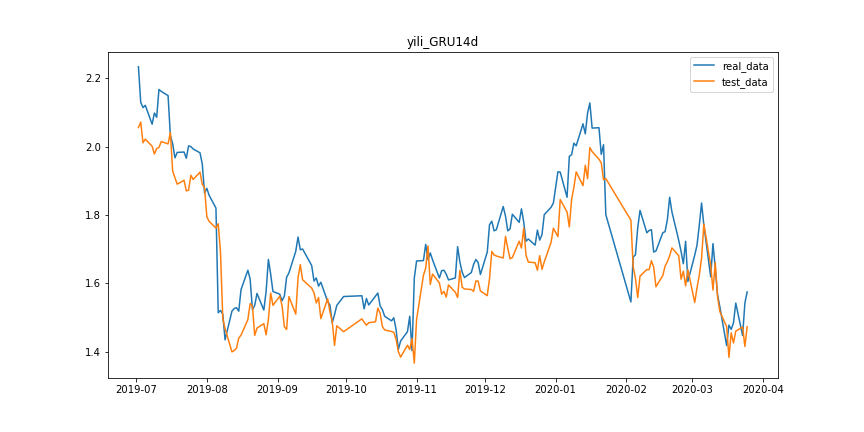
\includegraphics[width=4in]{yili_GRU14d.png} 
    \label{fig:yili_14d} %% label for first subfigure
  } 
  \subfigure[Extend text data]{ 
    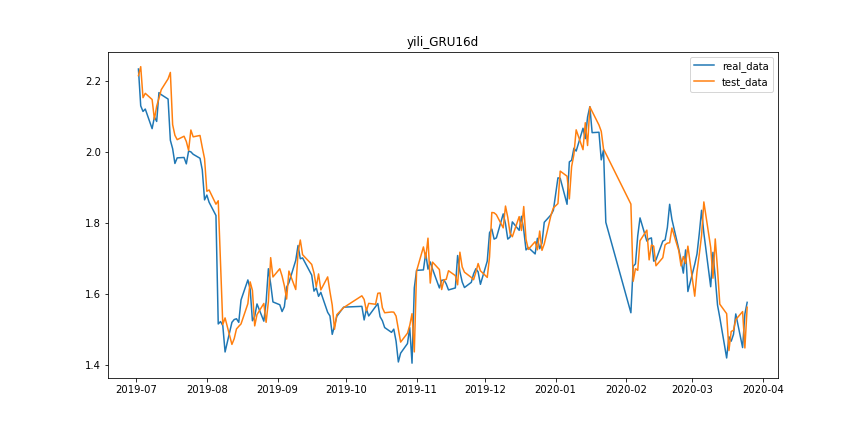
\includegraphics[width=4in]{yili_GRU16d.png} 
    \label{fig:yili_16d} %% label for second subfigure 
  } 
  \caption{Yili's prediction result} 
  \label{fig:Yili} %% label for entire figure 
\end{figure}

\begin{figure}
\centering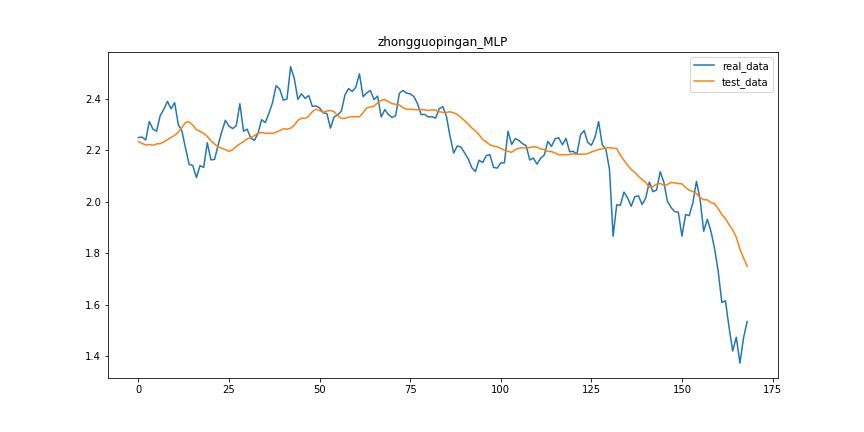
\includegraphics[width=4in]{zhongguopingan_MLP.png}
\caption{MLP} \label{fig:MLPres}
\end{figure}

\section{Conclusion}
Our paper focused on stock prediction problem on Chinese data. Specifically, we aimed to tackle a challenge lying on sentiment analysis in this problem, due to the lack of data source and labeled training data, which is a crucial part to train language processing model. We applied a semi-supervised learning method to generate training data and use the data to train BERT, a leading NLP model provided by Google. Based on this method, we successfully improved sentiment analysis efficiency on Chinese financial text data.

We further combined the sentiment data derived from our proposed method with stock transaction data and passed them into several neural network models to testify our method’s efficiency when used into stock prediction problem. The experiment results successfully buttressed up our argument and also revealed its adaptability over different type of problems. 

We believed our method can be widely used in this field as an effective way to supplement the insufficiency of labeled data and serve as a foundation for future works to generate more valuable insights.




%
% ---- Bibliography ----
%
% BibTeX users should specify bibliography style 'splncs04'.
% References will then be sorted and formatted in the correct style.
%
% \bibliographystyle{splncs04}
% \bibliography{mybibliography}
%
\begin{thebibliography}{8}
\bibitem{MACD}
Appel, Gerald: Technical analysis: power tools for active investors. FT Press, (2005)

\bibitem{autoregression}
Li, Lili and Leng, Shan and Yang, Jun and Yu, Mei.: Stock Market Autoregressive Dynamics: A Multinational Comparative Study with Quantile Regression. Mathematical Problems in Engineering (PT.10), 1285768.1--1285768.15 (2016)

\bibitem{ML-autoregression}
Nayak, Rudra Kalyan and Mishra, Debahuti and Rath, Amiya Kumar.: A Na?ve SVM-KNN based stock market trend reversal analysis for Indian benchmark indices. Applied Soft Computing \textbf{35}, 670--680 (2015)

\bibitem{neuralnetwork}
S. {Selvin} and R. {Vinayakumar} and E. A. {Gopalakrishnan} and V. K. {Menon} and K. P. {Soman}: Stock price prediction using LSTM, RNN and CNN-sliding window model. 2017 International Conference on Advances in Computing, Communications and Informatics (ICACCI), 1643--1647 (2017)

\bibitem{SFM}
Hu, Hao and Qi, Guo-Jun: State-Frequency Memory Recurrent Neural Networks. Proceedings of the 34th International Conference on Machine Learning - Volume 70. JMLR.org, Sydney, NSW, Australia, 1568–1577 (2017)

\bibitem{investmentbev}
Chen, Chi and Zhao, Li and Bian, Jiang and Xing, Chunxiao and Liu, Tie-Yan. : Investment behaviors can tell what inside: Exploring stock intrinsic properties for stock trend prediction. Proceedings of the 25th ACM SIGKDD International Conference on Knowledge Discovery \& Data Mining. 2376--2384 (2019)

\bibitem{dlnews}
Xiao, Ding and Yue, Zhang and Liu, Ting and Duan, Junwen. Deep Learning for Event-Driven Stock Prediction. International Conference on Artificial Intelligence. (2015)

\bibitem{sentimentprediction}
Si, Jianfeng and Mukherjee, Arjun and Bing, Liu and Pan, Jialin and Li, Huayi. Exploiting Social Relations and Sentiment for Stock Prediction. Emnlp. (2014)

\bibitem{finbert}
Araci, Dogu. FinBERT: Financial Sentiment Analysis with Pre-trained Language Models. (2019)

\bibitem{semi-supervised}
Dasgupta, Sajib and Ng, Vincent. Mine the Easy, Classify the Hard: A Semi-Supervised Approach to Automatic Sentiment Classification. ACL 2009, Proceedings of the 47th Annual Meeting of the Association for Computational Linguistics and the 4th International Joint Conference on Natural Language Processing of the AFNLP, 2-7 August 2009, Singapore. (2017)

\end{thebibliography}
\end{document}
